For at kunne komprimere en besked er det vigtigt at kende til teknologien bag sms'er.

Den teknologi som anvendes i moderne telefoner hedder GSM (Global System for Mobile Communications), som er en 2G standard. Denne teknologi g�r det muligt at benytte sig af sms'er.\cite{GSM_term}

For at et computersystem skal have muligheden for at kunne printe tegn til sk�rmen, er det n�dvendig at repr�sentere disse tegn med hver sit tal. Disse tal har man bestemt i en standard, som betyder at alle skal benytte de samme tal, for de samme tegn, og derved g�re det lettere for programm�rerne af softwaren der benytter disse tegn. Den mest brugte standard indenfor tegns�t, som dette kaldes, er unicode.\cite{UNICODE_standard}

I mobiler der g�r brug af GSM, kan der til sms'er, benyttes et tegns�t kaldt GSM 03.38. Dette tegns�t kan kodes i en r�kke alfabeter, hvor standard alfabetet GSM 7 bit er et krav ved skabelse af mobiltelefoner.\cite{GSM_7_bit}

\begin{figure}[H]
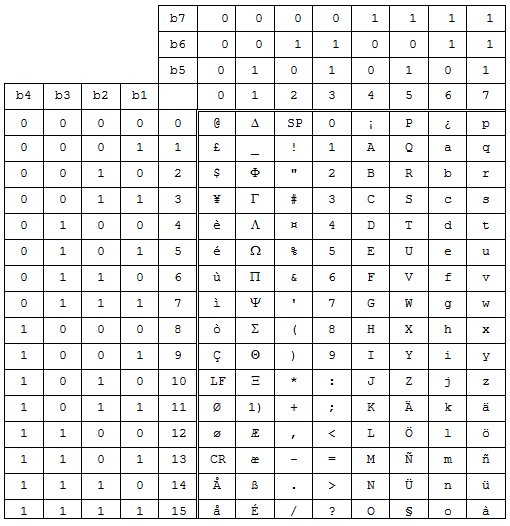
\includegraphics[width=\linewidth]{Billeder/tegnsaet.png}
\caption{Her ses et skema af GSM 7 bit alfabetet.}
\end{figure}

I dette skema symboliserer den vandrette linje, over den stiplede linje, det foerste ciffer, mens den lodrette kolonne er andet ciffer. F.eks hvis man skal printe tegnet A, har den en talvaerdi paa 42. Ved b1 til b7 vises ogsaa den binaere talvaerdi.
